\documentclass[tikz]{standalone}

\usepackage{fontspec}
\setmainfont[Ligatures=TeX, Mapping=tex-text]{Lato}
\setmonofont{FreeMonoBold}
\usepackage{tikz}
\usetikzlibrary{arrows.meta}
\usepackage{xfp}

\begin{document}
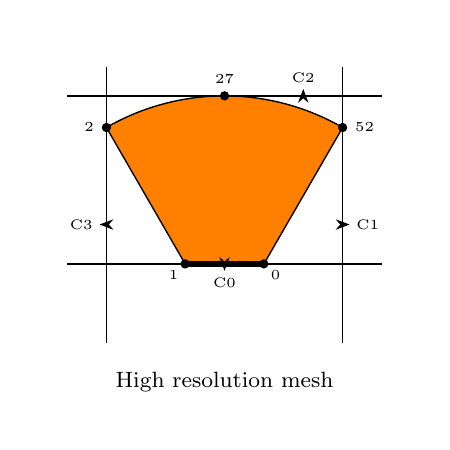
\begin{tikzpicture}

\def\width{5}
\def\height{5}
\def\ox{\fpeval{\width /2}}
\def\oy{\fpeval{\height /2}}

\tiny
\path [use as bounding box] (0,0) rectangle (\width,\height);

% SHAPE
\filldraw [line width=0.5pt, fill=orange] (\ox,\oy) ++(0,-0.5)
	+(0.5,0) node[draw, fill=black, circle, inner sep=1pt] {} node[below right] {0} --
	+(-0.5,0) node[draw, fill=black, circle, inner sep=1pt] {} node[below left] {1} --
	+(-1.5,1.73205) node[draw, fill=black, circle, inner sep=1pt] {} node[left=2pt] {2} --
	+(-1.44297,1.76415) --
	+(-1.38525,1.79501) --
	+(-1.32687,1.82459) --
	+(-1.26785,1.8529) --
	+(-1.20824,1.87991) --
	+(-1.14805,1.90561) --
	+(-1.08731,1.93) --
	+(-1.02606,1.95305) --
	+(-0.964318,1.97476) --
	+(-0.902117,1.99513) --
	+(-0.839487,2.01412) --
	+(-0.776457,2.03175) --
	+(-0.713058,2.048) --
	+(-0.649319,2.06286) --
	+(-0.585271,2.07633) --
	+(-0.520945,2.0884) --
	+(-0.45637,2.09906) --
	+(-0.391579,2.10831) --
	+(-0.326601,2.11614) --
	+(-0.261467,2.12256) --
	+(-0.196209,2.12755) --
	+(-0.130858,2.13112) --
	+(-0.0654447,2.13326) --
	+(0,2.13397) node[draw, fill=black, circle, inner sep=1pt] {} node[above=2pt] {27} --
	+(0.0654447,2.13326) --
	+(0.130858,2.13112) --
	+(0.196209,2.12755) --
	+(0.261467,2.12256) --
	+(0.326601,2.11614) --
	+(0.391579,2.10831) --
	+(0.45637,2.09906) --
	+(0.520945,2.0884) --
	+(0.585271,2.07633) --
	+(0.649319,2.06286) --
	+(0.713058,2.048) --
	+(0.776457,2.03175) --
	+(0.839487,2.01412) --
	+(0.902117,1.99513) --
	+(0.964318,1.97476) --
	+(1.02606,1.95305) --
	+(1.08731,1.93) --
	+(1.14805,1.90561) --
	+(1.20824,1.87991) --
	+(1.26785,1.8529) --
	+(1.32687,1.82459) --
	+(1.38525,1.79501) --
	+(1.44297,1.76415) --
	+(1.5,1.73205) node[draw, fill=black, circle, inner sep=1pt] {} node[right=2pt] {52} --
	cycle;

% PORTS
\draw [line width=2pt] (\ox,\oy) ++(0,-0.5) +(-0.5,0) -- +(0.5,0);

% MESH
\draw [line width=0.5pt] (\ox,\oy) ++(0,-0.5) +(-2,0) -- +(2,0);
\draw [line width=0.5pt] (\ox,\oy) ++(0,-0.5) ++(0,2.13397) +(-2,0) -- +(2,0);
\draw [line width=0.5pt] (\ox,\oy) ++(-1.5,0) +(0,-1.5) -- +(0,2);
\draw [line width=0.5pt] (\ox,\oy) ++(1.5,0) +(0,-1.5) -- +(0,2);
\path [tips, -{Stealth[length=5pt]}](\ox,\oy) ++(0,-0.5) -- +(0,-2.5pt) node[below] {C0};
\path [tips, -{Stealth[length=5pt]}](\ox,\oy) ++(1.5,0) -- +(2.5pt,0) node[right] {C1};
\path [tips, -{Stealth[length=5pt]}](\ox,\oy) ++(1,-0.5) ++(0,2.13397) -- +(0,2.5pt) node[above] {C2};
\path [tips, -{Stealth[length=5pt]}](\ox,\oy) ++(-1.5,0) -- +(-2.5pt,0) node[left] {C3};

% NOTE
\draw (\ox,\oy) ++(0,-2) node {\footnotesize High resolution mesh};

\end{tikzpicture}
\end{document}
